\section{Challenges for imaging MeerKAT data} \label{meerkat}
We introduced the basic measurement equation and the imaging problem for Radio Interferometers. MeerKAT introduces a variety of new challenges for image reconstruction. In this work, we limit the scope to the third Fourier term of wide field of view imaging, and discuss the basics of calibration. Both directly affect how the reconstruction algorithm deals with the Fourier Transform and the wider architecture of the reconstruction. In this section, we look at the wide field of view measurement equation, discuss the basics of calibration and how they are solved in the Major Cycle architecture.


\subsection{Wide Field of View Imaging and the third Fourier dimension} \label{meerkat:wof}
In wide field of view imaging, the simplifications we could make from the basic measurement equation \eqref{intro:basic} do not hold. The Visibility space of an interferometer actually has a third $w$-term. This leads us to the wide field of view measurement equation \eqref{meerkat:ftsphere}.

\begin{equation}\label{meerkat:ftsphere}
V(u, v, w) = \int\int \frac{I(x, y)}{\sqrt{1 - x^2 - y ^2}} e^{2 \pi i [ux+vy+ w(\sqrt{1 - x^2 - y ^2} - 1)]} \: dx \: dy
\end{equation}

For a small field of view, the term  $\sqrt{1 - x^2 - y ^2} \approx 1$, which simplifies to our original \eqref{intro:basic}, we can ignore the $w$-term and use the two dimensional Fourier transform. Older interferometers typically created small field of view observations, where the basic measurement equation was accurate enough. But MeerKAT produces wide field of view observations. The $w$-term cannot be ignored anymore and has to be corrected. The figure \ref{meerkat:wcorrection} shows the effect of ignoring the $w$-term for wide-field of view observations. The image gets more distorted away from the center. Emissions at the edges of the image get "torn" apart.

\begin{figure}[h]
	\centering
	\begin{subfigure}[b]{0.45\linewidth}
		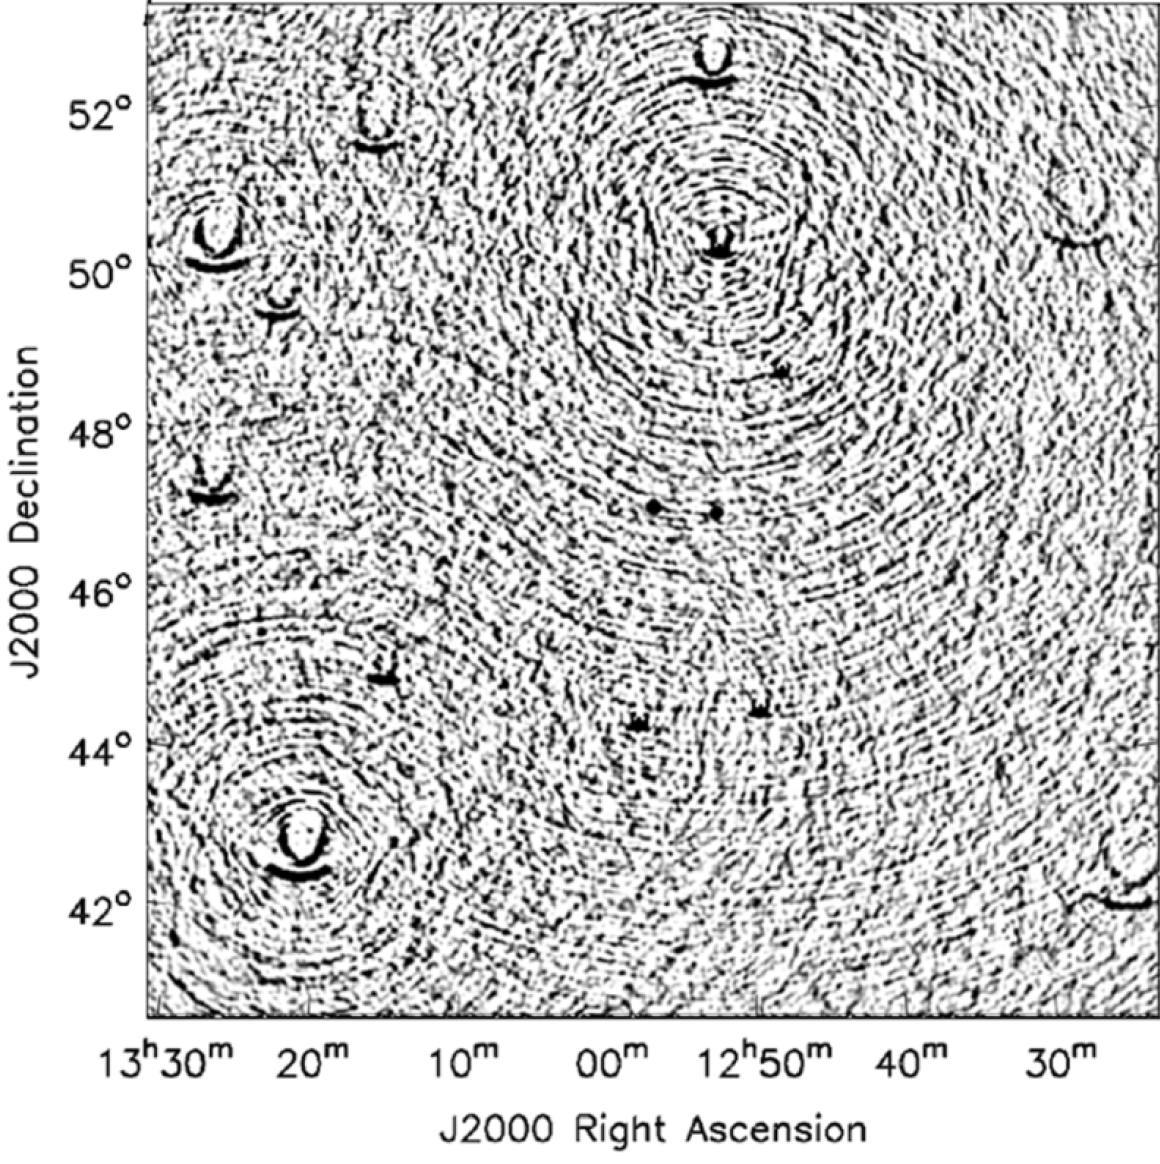
\includegraphics[width=\linewidth]{./chapters/03.challenges/w-no-correction.png}
		\caption{2D Fourier Transform.}
		\label{meerkat:2dfft}
	\end{subfigure}
	\begin{subfigure}[b]{0.45\linewidth}
		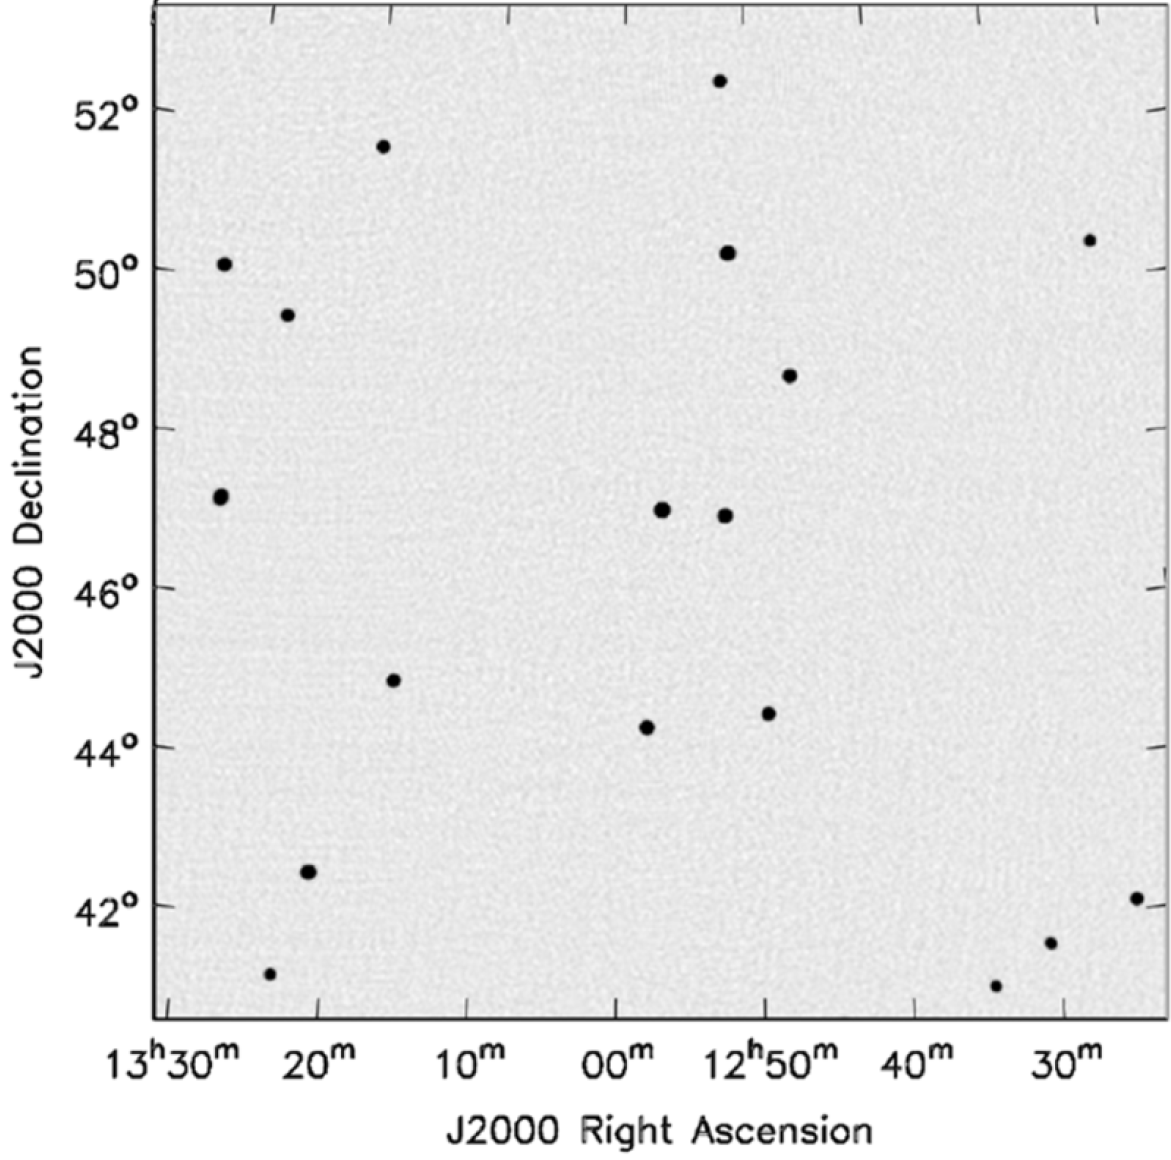
\includegraphics[width=\linewidth]{./chapters/03.challenges/w-correction.png}
		\caption{Fourier Transform with $w$-correction.}
		\label{meerkat:wcorrection}
	\end{subfigure}
	\caption{Celestial sphere distortion on simulated data. Source: \cite{cornwell2008noncoplanar}}
	\label{meerkat:wdistortion}
\end{figure}

Let us look at the wide field of view measurement equation \eqref{meerkat:ftsphere} in detail and explain this phenomenon. We see that the image $I(x,y)$ still two dimensional, even with a three dimensions in Visibility space. The observed image of the interferometer is not on a flat plane, but on a curved surface(hence the $w$-term)\cite{mcewen2011compressed}. More precisely, the instrument looks at the inside wall of the celestial sphere. The two dimensional Fourier transform approximates the curved surface with a flat plane, where the tangent point is typically the image center. The further away we move from the tangent point, the more distortion gets added by the curvature, represented by the term $\sqrt{1 - x^2 - y ^2}$. The curve adds a phase shift the further away we move from the tangent point. If the reconstruction algorithm ignores the $w$-component for a wide field of view, the phase-shift gets severe enough to decorrelate the Visibilities, "tearing" apart the image structures of \eqref{meerkat}.

The effect of the $w$-term is one example of a Direction Dependent Effect (DDE). Wide field of view imaging introduces a number of DDE's, like distortions from the ionosphere and bleed over from different polarization. Correcting for the DDE in the Major Cycle architecture is under research\cite{intema2009ionospheric}, and is therefore out of scope for this project. We only correct for the $w$-term which directly influences the Fourier Transform and the architecture of reconstruction algorithms. 


\subsubsection{State of the art: $w$-stacking algorithm}
The third Fourier breaks the two dimensional relationship between image and Visibilities, which keeps us from using the non-uniform FFT in the Major Cycle architecture. Before the $w$-stacking algorithm was developed, a wide field of view image was faceted into image patches where the $w$-term could be approximated with the small field of view measurement equation. $w$-stacking is the state-of-the-art way of approximating for the $w$-correction in an efficient manner. It calculates a $w$-corrected dirty image from three dimensional Visibilities.

\begin{wrapfigure}{r}{0.7\textwidth}
	\centering
	\vspace{-10pt}
	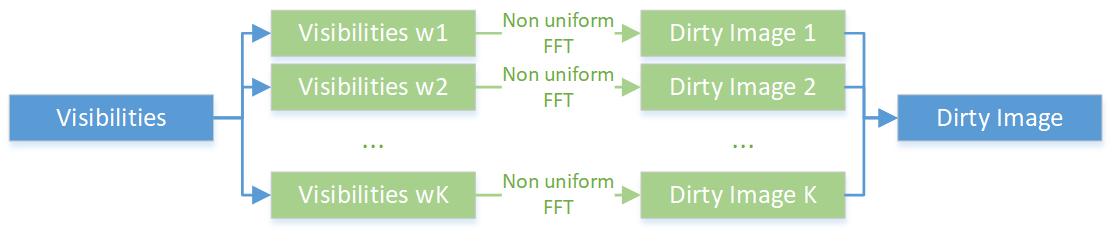
\includegraphics[width=1.0\linewidth]{./chapters/03.challenges/w-stacks.png}
	\caption{The Major Cycle Framework}
	\label{meerkat:w-stacks}
	\vspace{-10pt}
\end{wrapfigure}

The $w$-stacking algorithm, shown in figure \ref{meerkat:w-stacks} replaces the non-uniform FFT. It groups the Visibilities with similar $w$-term into the same layer. Multiple layers are then stacked and transformed independently with the non-uniform FFT. For each stack, the $w$-correction is performed for the center $w$-component. The last step is summing over all stacked images, giving us the final dirty image. From here on a standard CLEAN deconvolution, or a Compressed Sensing algorithm can search for the observed image.

Afterwards, the whole process is reversed. The image gets copied back into the stacks, the $w$-correction gets reversed and the non-uniform FFT calculates the Visibilities per stack.

If we choose uses as many stacks as Visibilities, we end up with an exact $w$-corrections. In practice, many Visibilities have a similar $w$-term. $w$-stacking approximates the correction and allows the Major Cycle to distribute the forward- and backwards non-uniform FFT to a certain extend.

\subsection{Basic Calibration and Self-Calibration}
The Visibilities measured by a Radio interferometer require calibration before an image can be reconstructed.
Radio Interferometer require calibration of their complex valued Visibility measurements. The amplitude and phase of a Visibility is subject to 

Before the advent of self-calibration, the calibration terms were 
Complex gain term. Corrects amplitude and phase. 

Traditional Calibration

A calibration source close by, with a known brightness. Phase and amplitude calibration was done before image reconstruction. For older interferometers, there was a very limited number of calibration terms to solve.


but again effects of wide field of view also increase the number of necessary calibration terms. The advent of self calibration, in which the image reconstruction was used to solve for both, the observed image and the calibration of the instrument.

Self calibration with the major cycle algorithm and a CLEAN deconvolution.

Initial phase calibration
Shallow clean
phase calibration
deep clean
phase and amplitude calibration
deep clean
reconstruction






